% !TEX TS-program = xelatex+makeindex+bibtex+shellescape
% !TEX encoding = UTF-8 Unicode

% Copyright 2024 Advaith Menon/GaTech

% Permission is hereby granted, free of charge, to any person obtaining
% a copy of this software and associated documentation files (the 
% "Software"), to deal in the Software without restriction, including
% without limitation the rights to use, copy, modify, merge, publish,
% distribute, sublicense, and/or sell copies of the Software, and to
% permit persons to whom the Software is furnished to do so, subject
% to the following conditions:

% The above copyright notice and this permission notice shall be
% included in all copies or substantial portions of the Software.

% THE SOFTWARE IS PROVIDED “AS IS”, WITHOUT WARRANTY OF ANY KIND,
% EXPRESS OR IMPLIED, INCLUDING BUT NOT LIMITED TO THE WARRANTIES
% OF MERCHANTABILITY, FITNESS FOR A PARTICULAR PURPOSE AND
% NONINFRINGEMENT. IN NO EVENT SHALL THE AUTHORS OR COPYRIGHT
% HOLDERS BE LIABLE FOR ANY CLAIM, DAMAGES OR OTHER LIABILITY,
% WHETHER IN AN ACTION OF CONTRACT, TORT OR OTHERWISE, ARISING
% FROM, OUT OF OR IN CONNECTION WITH THE SOFTWARE OR THE USE OR
% OTHER DEALINGS IN THE SOFTWARE.

% Initial conditions, system and surroundings, FBD

\subsection{Initial Conditions}
\begin{frame}{Initial Conditions}
	\begin{itemize}
	\item Initial position, \(\vec{r}_i = 0\hat{i} + 1.12\times 10^{-2} \hat{j} + 0\hat{k}\ \mathrm{m} \)
	\item Mass of the ball, \(m_{ball} = 4.6\ \mathrm{g} = 4.6 \times 10^{-3}\ \mathrm{kg}\)
	\end{itemize}
\end{frame}

\begin{frame}{System and Surroundings}
	\begin{itemize}
	\item \textbf{System:} Paper ball (hereafter referred to as `object')
	\item \textbf{Surroundings:} Everything else (table, air, etc.)
	\end{itemize}
\end{frame}

\begin{frame}{Free-Body Diagram}
    \begin{center}
	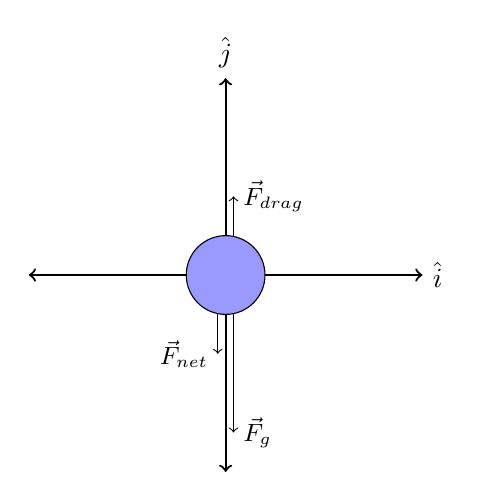
\begin{tikzpicture}[scale=0.5]
    % axes
    % \draw[step=1cm,gray,very thin] (-5, -5) grid (5, 5);
    \draw[thick,->] (0, 0) -- (0, 5) node[anchor=south] {\(\hat{j}\)};
    \draw[thick,->] (0, 0) -- (5, 0) node[anchor=west] {\(\hat{i}\)};
    \draw[thick,->] (0, 0) -- (0, -5);
    \draw[thick,->] (0, 0) -- (-5, 0);
    % forces
    \draw[->] (0.2, 0) -- (0.2, -4) node[font=\small, anchor=west] {\(\vec{F}_g\)};
    \draw[->] (0.2, 0) -- (0.2, 2) node[font=\small, anchor=west] {\(\vec{F}_{drag}\)};
    \draw[->] (-0.2, 0) -- (-0.2, -2) node[font=\small, anchor=east] {\(\vec{F}_{net}\)};
    % ball
    \fill[blue!40!white, draw=black] (0, 0) circle (1cm);
    \end{tikzpicture}
    \end{center}
\end{frame}